\documentclass[12pt,a4paper]{article}
\usepackage[T1]{fontenc}
\usepackage{lmodern}
\usepackage[german]{babel}
\usepackage[utf8]{inputenc}  
\usepackage{microtype} 
\usepackage{graphicx}

\title{Colliding Empires - Spielregeln}
\author{Gruppe - 12}
\date{\today}

\begin{document}

\makeatletter
    \begin{titlepage}
        \begin{center}
            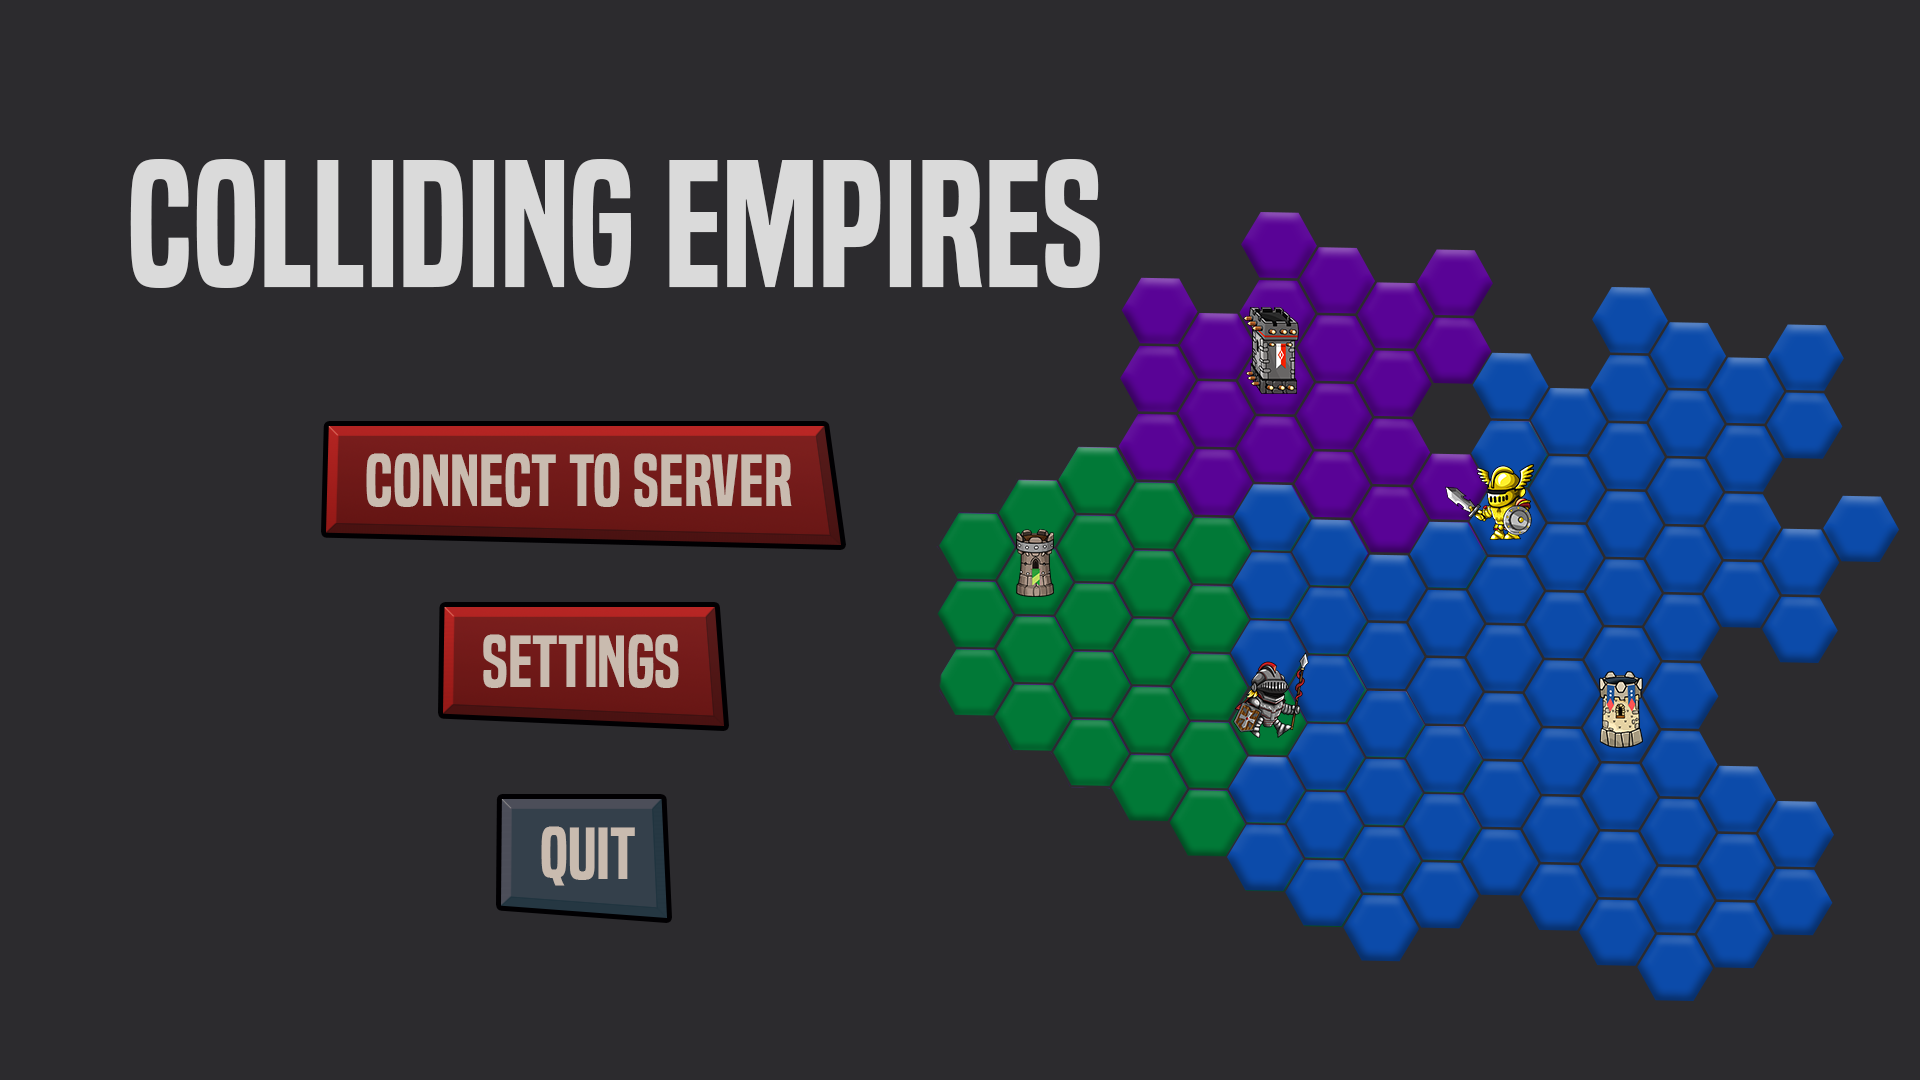
\includegraphics[width=1.0\linewidth]{img/titleimage.png}\\[5ex]
            {\huge \bfseries  \@title }\\[2ex] 
            {\LARGE  \@author}\\[50ex] 
            {\large \@date}
        \end{center}
    \end{titlepage}
\makeatother    
    
\newpage
\tableofcontents
\newpage

\section{Das Spielprinzip}

Bei \glqq Colliding Empires\grqq  kämpfen 4 Spieler um die Herrschaft einer Karte, die aus sechseckigen Feldern besteht. Jeder Spieler hat seine eigene Farbe, in der die sich im Besitz des jeweiligen Spielers befindlichen Felder, sowie dessen Gebäude und Einheiten eingefärbt werden.

Die Spiel unterteilt sich in Runden. Zu Beginn wird ein zufällig gewählter Spieler gewählt, der in der ersten Runde das Spiel eröffnet. Während einer Runde kann der Spieler, der an der Reihe ist, gültige Spielzüge ausführen, also hat die Wahl mit seinen vorhandenen Recourcen(Münzen) Gebäude zu bauen, Einheiten zu kaufen oder eben diese zu bewegen um neues Land zu erobern.

\subsection{Das Ziel}
Das Ziel von Colliding Empires ist die Eroberung der gesamten Spielkarte oder das Erobern aller gegnerischer Spielfelder. Ist dieses Ziel erreicht wird das Spiel sofort beendet und der Spieler, der die gesamte Karte erobert hat, ist der Gewinner.

\section{Spielablauf}

Ist ein Spieler an der Reihe, so hat er ein Zeitlimit um Aktionen durchzuführen, in einer Spielrunde gilt \textbf{folgender Ablauf}:

\begin{itemize}
	\item	Der Spieler erhält eine bestimmte Anzahl Münzen 
	\item	Der Spieler führt gültige Spielzüge aus
	\item	Der Spieler beendet seinen Zug oder das Zeitlimit läuft ab
\end{itemize}

Nun ist der nächste Spieler an der Reihe. Dieser Ablauf setzt sich fort bis das Ziel des Spiels erreicht ist. Das Spiel wird dann sofort beendet und man gelangt zurück in die Lobby.

\section{Spielregeln}

\subsection{Münzen}
Münzen sind die Recource in \glqq Colliding Empires!\grqq Mit Ihnen kann ein Spieler Einheiten und Gebäude kaufen. Am Anfang jedes Spielzuges kriegt ein Spieler Münzen auf sein Konto gutgeschrieben. Eroberte Felder und spezielle Gebäude generieren Münzen, Einheiten verbrauchen Münzen pro Runde.

Ein Spieler kann nur so viele Einheiten bauen bis die Differenz zwischen Einkommen und Ausgaben minimal ist. 

\subsection{Gebäude und Felder}
Jeder Spieler startet mit 5 Feldern in seiner Farbe und einem Rathaus.
\begin{table}[h!]
\resizebox{0.7\textwidth}{!}{\begin{minipage}{\textwidth}
\begin{tabular}{c|c|c|c}
\textbf{Art} & \textbf{Kosten} & \textbf{generierte Münzen pro Runde} & \textbf{Sonderfunktion} \\
\hline
Farm & 12 (+2 pro vorhandener Farm) & 3 & - \\
\hline
Rathaus & Nur Initial & - & anliegende Felder Kampfstufe + 1  \\
\hline
Turm & 15 & - & anliegende Felder Kampfstufe + 1 \\
\hline
Feld & Erobern & 1 & generiert nur sofern kein Baum \\
\end{tabular}
\end{minipage}}
\end{table}

Ein Feld mit einer Farm generiert 4 Münzen pro Runde und nicht 3! Das Feld wird in diesem Fall also mitgezählt. Genauso erhält der Spieler Münzen für eigene Felder obwohl sich Gebäude auf diesen befinden.  

\subsection{Einheiten}
Einheiten sind dazu da Felder zu erobern und gewachsene Bäume von bereits eroberten Feldern zu beseitigen, da diese sonst keine Münzen mehr generieren. Sie verbrauchen jede Runde eine bestimmte Anzahl an Münzen. Jede Einheit hat eine Bewegungsreichweite von maximal 6 Feldern. Außerdem besitzen Einheiten eine Kampfstufe, die wichtig wird wenn es um die Eroberung und Verteidigung von Spielfeldern geht.

Hat man einen einfachen Soldat gekauft, so kann man ihn aufwerten um seine Kampfstufe zu erhöhen. Einen Soldaten höherer Stufe kann man also nicht direkt erwerben! 

\begin{table}[h!]
\centering
\begin{tabular}{c|c|c|c}
\textbf{Art} & \textbf{Kosten} & \textbf{Kosten pro Runde} & \textbf{Kampfstufe} \\
\hline
Einfacher Soldat & 10 & 1 & 1 \\
\hline
+ Speer & 20 & 5 & 2 \\
\hline
+ Schild \& Speer & 30 & 10 & 3 \\
\hline
+ Schild \& Speer\& Helm & 40 & 20 & 4 \\
\end{tabular}
\end{table}
\newpage
\subsection{Bewegen und Erobern}
Einheiten können sich nur auf Felder bewegen dessen Kampfstufe niedriger ist als Ihre Eigene. 
Ein Feld erhält Kampfstärke durch die Einheit, die sich auf ihm befindet, so wie durch angrenzende Türme oder Rathäuser(Pro Turm oder Rathaus +1).

Bewegt sich eine Einheit auf ein Feld mit einem Gegnerischen Gebäude so wird dieses zerstört und die Einheit besetzt dieses! Eigene Einheiten können sich nicht auf eigene Felder mit Gebäuden bewegen!

Hat sich eine Einheit auf ein Feld bewegt so gehört dieses Feld ab sofort automatisch dem Spieler, dem die erobernde Einheit gehört.

\subsection{Bäume}
Im Verlauf des Spiels können auf dem Spielfeld zufällig Bäume wachsen. Diese verhindern, dass dieses Spielfeld, sofern im eigenen Besitz, Münzen generiert. Um das Feld wieder freizugeben und den Baum zu entfernen muss sich eine Einheit auf dieses Feld bewegen. Die Entfernung geschieht also immer wenn sich eine Einheit auf das Feld bewegt.
\end{document}